
\chapter{\label{chap:res}Results}%


\section{\label{sec:res_fig_plot}Bending Loss Experiment}

\subsection{Experimental Data}
\begin{table}[H]
         \centering
        \begin{tabular}{|c|c|c|}
             \hline
        \textbf{Diameter (mm)} & \textbf{Number of Turns} & \textbf{Current (mA)} \\
        \hline
        35 & 5 & 1.2 \\
        35 & 4 & 1.4 \\
        35 & 3 & 1.5 \\
        35 & 2 & 1.6 \\
        35 & 1 & 1.9 \\
        \hline
        45 & 5 & 1.7 \\
        45 & 4 & 1.7 \\
        45 & 3 & 1.8 \\
        45 & 2 & 1.8 \\
        45 & 1 & 2.0 \\
        \hline
        55 & 1 & 2.5 \\
        55 & 2 & 2.2 \\
        55 & 3 & 2.4 \\
        55 & 4 & 2.3 \\
        55 & 5 & 2.3 \\
        \hline
        65 & 1 & 2.7 \\
        65 & 2 & 2.6 \\
        65 & 3 & 2.5 \\
        65 & 4 & 2.4 \\
        65 & 5 & 2.4 \\
        \hline
    \end{tabular}
    \caption{Data of Bending Loss Expt.}
    \end{table}

     \begin{table}[H]
    \centering
    \begin{tabular}{|c|c|}
        \hline
        \textbf{Diameter (mm)} & \textbf{Weighted Mean Current (mA)} \\
            \hline
            35 & 1.41 \\
            45 & 1.75 \\
            55 & 2.29 \\
            65 & 2.46 \\
            \hline
        \end{tabular}
        \caption{Weighted Mean for each Diameter}
    \end{table}
\subsection{Plots}
\begin{figure}[!h]
        \centering
        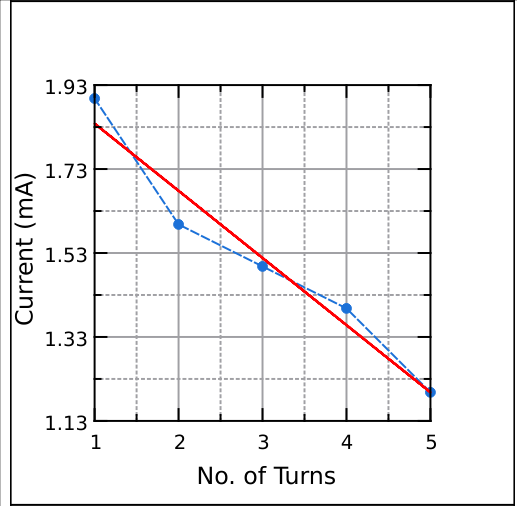
\includegraphics[width = 11cm]{images/BL1.png}
        \caption{Bending the Fiber on 35 mm Diameter Circle(\textcolor{red}{Red Line} represents linear fitting)}
    \end{figure}
    \begin{figure}
        \centering
        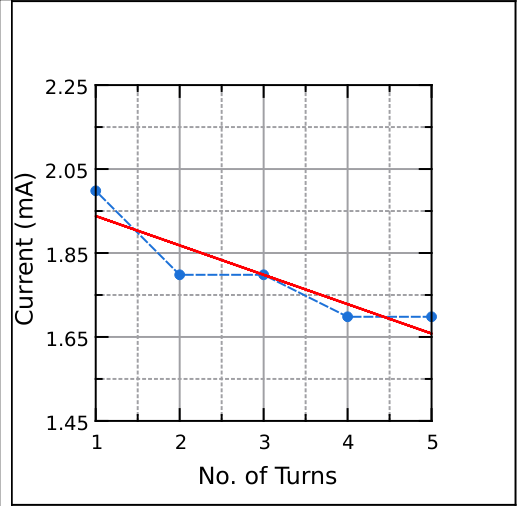
\includegraphics[width = 11cm]{images/BL2.png}
        \caption{Bending the Fiber on 45 mm Diameter Circle}
    \end{figure}
\begin{figure}
        \centering
        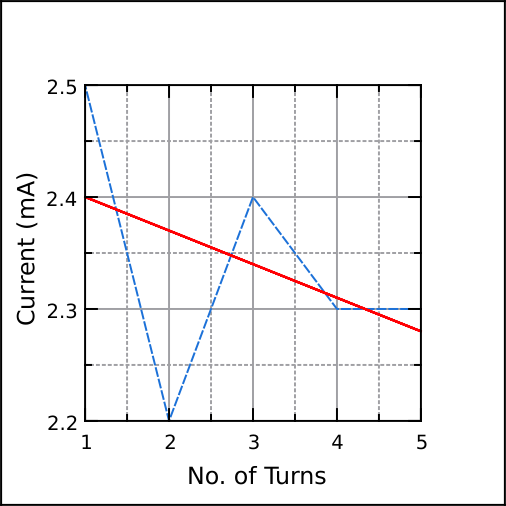
\includegraphics[width = 11cm]{images/BL3.png}
        \caption{Bending the Fiber on 55 mm Diameter Circle}
    \end{figure}
\begin{figure}
        \centering
        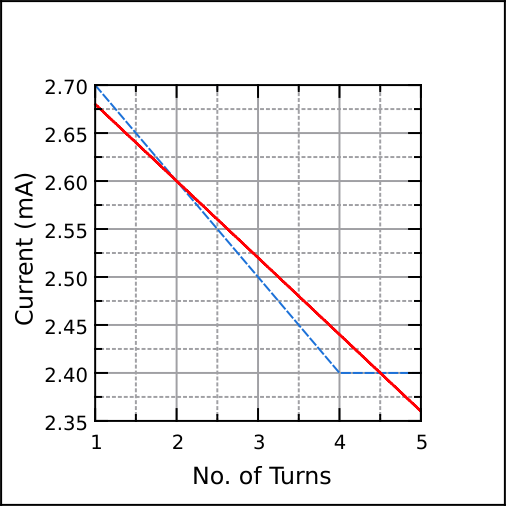
\includegraphics[width = 10cm]{images/BL4.png}
        \caption{Bending the Fiber on 65 mm Diameter Circle}
    \end{figure}
\begin{figure}
        \centering
        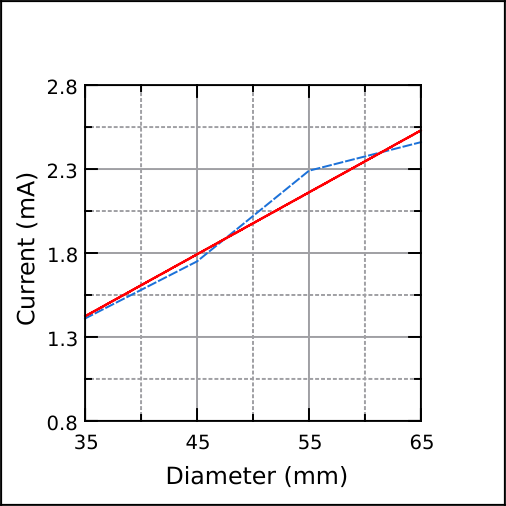
\includegraphics[width = 10cm]{images/BL_MEAN.png}
        \caption{Bending the Fiber on various Diameters(Weighted Mean)}
    \end{figure}
\pagebreak    
\section{Calculation of Numerical Aperature}
\subsection{Experimental Data}

    \begin{table}[htbp]
         \centering
        \begin{tabular}{|c|c|}
             \hline
             \textbf{Displacement (mm)} & \textbf{Current (mm)} \\
             \hline
                9 & 0 \\
                9.1 & 0 \\
                9.2 & 0 \\
                9.3 & 0.1 \\
                9.4 & 0.2 \\
                9.5 & 0.3 \\
                9.6 & 0.6 \\
                9.7 & 0.8 \\
                9.8 & 1.1 \\
                9.9 & 1.4 \\
                10 & 1.8 \\
                10.1 & 2.1 \\
                10.2 & 2.4 \\
                10.3 & 2.7 \\
                10.3 & 2.7 \\
                10.4&	3 \\ 
                10.5&	3.3 \\ 
                10.6&	3.5 \\
                10.7&	3.6 \\
                10.8&	3.5 \\
                10.9&	3.3 \\
                11	&3 \\
                11.1&	2.7 \\
                11.2&	2.3 \\
                11.3&	2 \\
                11.4&	1.7 \\
                11.5&	1.4 \\
                11.6&	1 \\
                11.7&	0.7 \\
                11.8&	0.5 \\
                11.9&	0.3 \\
                12	&0.1 \\
                12.1&	0 \\
            \hline
        \end{tabular}
        \caption{Table for Numerical Aperature}
    \end{table}
\subsection{Plots}
\begin{figure}[H]
        \centering
        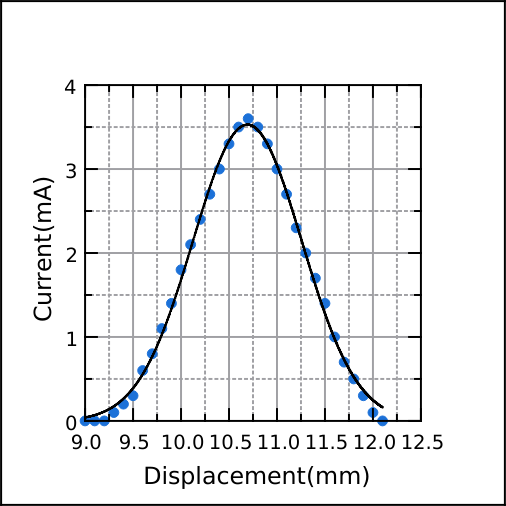
\includegraphics[width = 12 cm]{chapters/NA.png}
        \caption{Numerical Aperture Measurement(\textbf{Black Line}represents Gaussian fitting)}
    \end{figure}
    
\subsection{Calculations}

From the theory we have,
    So, the Acceptance angle is defined by \\
    $$ \theta_{a} = \tan^{-1}\frac{D}{Z}$$ \\
   
    Diameter of far field intensity at 5 percent intensity Micrometer reading (mm) level of the maximum attainable intensity (Mode Field Diameter)
    $$ D = (10.7 - 9.3) mm = 1.4  mm$$
    
    Here, the Acceptance angle is given by,
    $$ \theta_{a} = \tan^{-1}\left(\frac{1.4}{5.00}\right) $$
    $$ \theta_{a} = 15.64^{o}$$ \\
    So, the Numerical Aperture is given by,
    $$ NA = \sin{\theta_{a}} $$
    $$ NA = \sin{(15.64^{o})}$$
    $$ NA = 0.26 $$
   
\begin{itemize}

    \item \textbf{Error Calculation: }
    $$ \theta_{a} = \tan^{-1}\frac{D}{Z} \implies \tan\theta_{a} = \frac{D}{Z} $$ \\
    Now, differentiating this term, we get,
    $$ \sec^{2}(\theta_{a})  \Delta \theta_{a} = \frac{\Delta D}{z} - \frac{D \Delta Z}{Z^{2}} $$
    $$ \Delta \theta_{a} = \frac{1}{\sec^{2}(\theta_{a})}\left(\frac{\Delta D}{z} - \frac{D \Delta Z}{Z^{2}}\right) $$ \\
    $$ \Delta \theta_{a} = \frac{1}{\sec^{2}(15.64)}\left(\frac{0.01}{5} - \frac{1.4 \times 0.01}{5^{2}}\right) $$
    $$  \Delta \theta_{a} = \frac{1}{\sec^{2}(15.64)} \times 0.001^{o} $$
    $$ \Delta \theta_{a} = 1.08 \times 0.001^{o} $$
    $$ \Delta \theta_{a} = 0.001^{o} $$
    
    While calculating the Numerical Aperture, we get,
    $$ NA = \sin{(\theta_{a})}$$
    $$ \Delta(NA) = \cos{(\theta_{a}) \times \Delta\theta_{a}}$$
    $$ \Delta(NA) = \cos{(15.64^{o}) \times 0.001^{o}} $$
    $$ \Delta(NA) \approx 0.001^{o}$$
    
    \item \textbf{Final Results} \\
    Mode Field Diameter (D) = (1.4 $\pm$ 0.01) mm \\
    Acceptance Angle ($\theta_{a}$) = $15.64^{o} \pm 0.001^{o}$ \\
    Numerical Aperture (NA) = $10.17^{o} \pm 0.001^{o}$ \\

\end{itemize}

\section{Splice Loss Experiment}

\subsection{Experimental Data}
\begin{itemize}
    \item \textbf{Variation due to Tilt}
    \begin{table}[H]
    \centering
    \begin{tabular}{|c|c|}
        \hline
        \textbf{Angle (Degree)} & \textbf{Current (mA)} \\
        \hline
            -8 & 0 \\
            -7 & 0.1 \\
            -6 & 0.2 \\
            -5 & 0.2 \\
            -4 & 0.4 \\
            -3 & 0.4 \\
            -2 & 0.6 \\
            -1 & 0.7 \\
            0 & 0.7 \\
            1 & 0.7 \\
            2 & 0.6 \\
            3 & 0.5 \\
            4 & 0.4 \\
            5 & 0.3 \\
            6 & 0.1 \\
            7 & 0 \\
        \hline
        \end{tabular}
        \caption{Variation of Light Intensity with the angle between two fibers}
    \end{table}
\pagebreak
    \item \textbf{Variation due to Lateral Offset}
    \begin{table}[H]
    \centering
    \begin{tabular}{|c|c|}
        \hline
        \textbf{Displacement (mm)} & \textbf{Current (mA)} \\
        \hline
        5.0 & 0 \\
        5.1 & 0.1 \\
        5.2 & 0.2 \\
        5.3 & 0.3 \\
        5.4 & 0.3 \\
        5.5 & 0.4 \\
        5.6 & 0.4 \\
        5.7 & 0.5 \\
        5.8 & 0.5 \\
        5.9 & 0.6 \\
        6.0 & 0.6 \\
        6.1 & 0.6 \\
        6.2 & 0.5 \\
        6.3 & 0.5 \\
        6.4 & 0.4 \\
        6.5 & 0.4 \\
        6.6 & 0.3 \\
        6.7 & 0.3 \\
        6.8 & 0.2 \\
        6.9 & 0.1 \\
        7.0 & 0 \\
        \hline
    \end{tabular}
    \caption{Variation of Light Intensity with Lateral Offset between Two Fibers}
\end{table}
\pagebreak
\item \textbf{Variation of Light Intensity with End Separation(Air Gap)}
\begin{table}[H]
    \centering
    \begin{tabular}{|c|c|}
        \hline
        \textbf{End Separation (mm)} & \textbf{Current (mA)} \\
        \hline
       0 &	9.7\\
0.1	& 9.6\\
0.2	& 9.4\\
0.3	& 9.1\\
0.4	& 8.7\\
0.5	& 8.2\\
0.6	& 7.6 \\
0.7	&7\\
0.8	&6.5\\
0.9	&6\\
1	&5.5\\
1.1	&5\\
1.2	&4.6\\
1.3	&4.2\\
1.4	&3.9\\
1.5	&3.5\\
1.6	&3.2\\
1.7	&2.9\\
1.8	&2.7\\
1.9	&2.5\\
2	&2.3\\
2.1	&2.1\\
2.2	&2\\
2.3	&1.9\\
2.4	&1.8\\
2.5	&1.6\\
2.6	&1.5\\
2.7	&1.4\\
2.8	&1.3\\
2.9&	1.2\\
3&1.1\\
        \hline
    \end{tabular}
    \caption{Variation of Light Intensity with Lateral Offset between Two Fibers}
\end{table}
\end{itemize}

\subsection{Plots}
\begin{figure}[h]
        \centering
        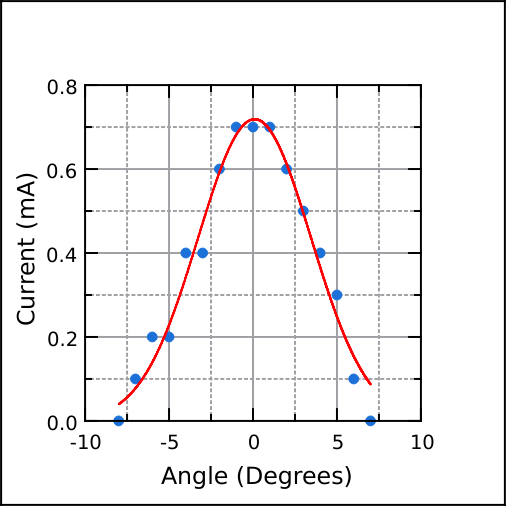
\includegraphics[width = 10 cm]{chapters/TILT.png}
        \caption{Variation due to Tilt(\textcolor{red}{Red Line} represents gaussian fitting)}
    \end{figure}
    \begin{figure}[h]
        \centering
        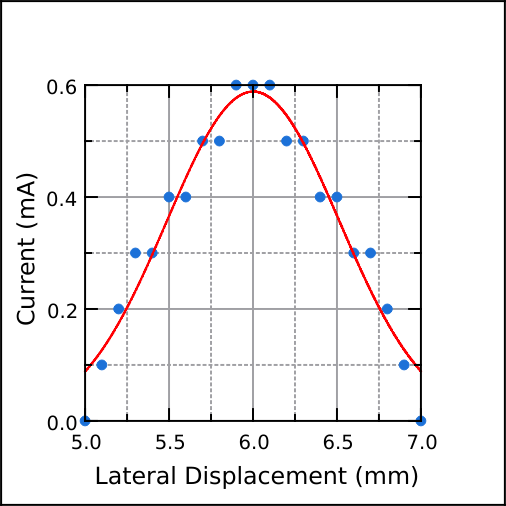
\includegraphics[width = 10 cm]{chapters/LO.png}
        \caption{Variation due to Lateral Offset}
    \end{figure}
    \begin{figure}
        \centering
        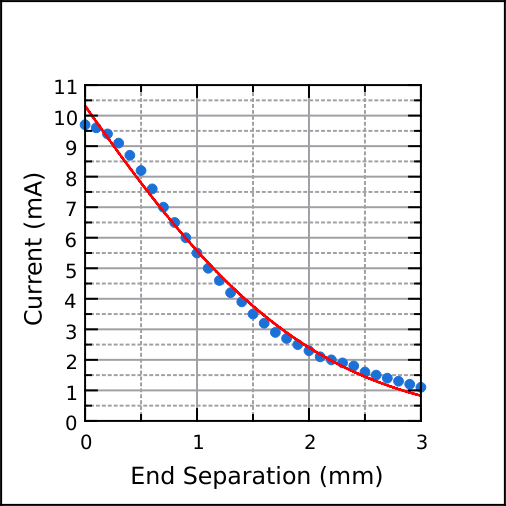
\includegraphics[width = 10 cm]{chapters/ES.png}
        \caption{Variation due to End Separation}
    \end{figure}
%\vspace{5cm}

